\label{sec:Grundlagen}
In diesem Kapitel werden die theoretischen Grundlagen, welche zum Verständnis der vorliegende Arbeit wichtig sind, beschrieben. Zu Beginn erfolgt ein Einstieg in künstliche neuronale Netze, anschließend werden die Hyperparameter und ihre Besonderheiten thematisiert. Dann folgt eine kurze Einführung in die Optimierungsverfahren. Abschließend werden die grundlegende Aspekte von Zufallssuche und Genetischen Algorithmen erläutert.

\section{Künstliche Neuronale Netze}
Im folgenden Unterkapitel wird zuerst der Aufbau eines Neurons erklärt. Anschließend wird der strukturelle Aufbau eines künstlichen neuronalen Netzes(KNN) näher gebracht. Es werden wichtige Funktionen wie die Verlustfunktion und die Fehlerrückführung erklärt. Zum Schluss wird auf die Hyperparameter, welche für die Arbeit essenziell sind, eingegangen.

Künstliche Intelligenz (engl. Artificial Intelligence) sorgte in den letzten Jahren für weitreichende Schlagzeilen. Im Detail versteckt sich hinter dieser künstlichen Intelligenz meist Maschinelles Lernen im speziellen tiefe künstliche neuronale Netze (engl. Deep Artificial neuronal Networks oder Deep Learning). Diese werden für Anwendungen mit großen Datenmengen eingesetzt, bspw. in Bereichen der Bildverarbeitung, Chatbots und Fahrassistenz Systemen. Beim Deep Learning werden die Funktionen durch ein Modell erlernt, welches künstliches neuronales Netz genannt wird. Dieser Begriff stammt ursprünglich aus der Neurobiologie. Bei den künstlichen neuronalen Netzen handelt es sich aber nicht um Nachbildungen des Gehirns, das natürliche Vorbild dient nur als Inspiration. In Abbildung \ref{fig:neural_network} ist so ein künstliches neuronales Netz zu sehen, wobei jede Schicht aus einzelnen Neuronen aufgebaut ist. Diese Schichten können dann Schichtweise zusammengefügt werden, wodurch ein Netz entsteht. Diese Verbindungen repräsentieren die Gewichte, über welche einem Netz, lineare als auch nicht lineare Zusammenhänge antrainiert werden. \cite[p.~11]{Silva2016}

\subsection{Aufbau eines Neurons}
\label{Aufbau eines Neurons}
Abbildung \ref{fig:neuron} zeigt ein Neuron. Dieses hat folgenden schematischen Aufbau Aufbau: Eingänge, Gewichte, Schwellwert, Aktivierungsfunktion und einen Ausgang. In den nachfolgenden Unterkapiteln werden diese ausführlich erklärt, Informationen dazu stammen wenn nicht anderweitig angegeben aus der Arbeit \cite[p.~12]{Silva2016}.

\begin{figure}[htb]
  \centering  
  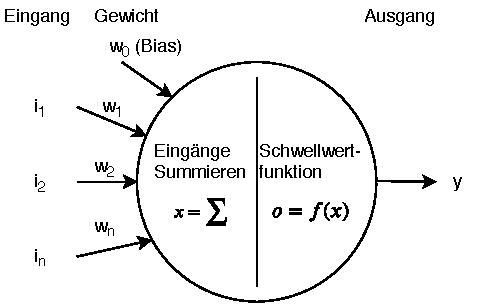
\includegraphics[scale=1]{img/neuron.pdf}
  \caption{Aufbau eines Neurons}
  \label{fig:neuron}
\end{figure}


\paragraph{Eingang}
Bei den Eingangswerten $i_1, ..., i_n$ handelt es sich um reelle Zahlen, diese werden mit den Gewichten $w_1, ..., w_n$ verrechnet. Ein Neuron hat meist mehrere Eingangsgrößen, welche alle zusammen mit den Gewichten und dem Schwellwert aufsummiert werden. Die Gewichte werden zufällig initialisiert und per Training verbessert, somit handelt es sich um angelernte Werte, welche durch die Fehlerrückführung (engl. Backpropagation) verbessert werden. Auf diese aufsummierten Ergebnisse wird anschließend ein Schwellwert (engl. Bias) $w_0$ gerechnet, dieser führt zu einem besseren Verhalten beim Trainieren. Beim Schwellwert handelt es sich auch um einen angelernten Wert. Dieser hilft die Flexibilität des Netzes zu erhöhen. Der Schwellwert sorgt dafür, dass ein Ausganswert erzeugt wird, auch wenn kein Eingangswert anliegt. Daraus ergibt sich folgende Übertragungsfunktion:

\begin{equation}
	x = \sum_{k=1}^n i_k * w_k + w_0 \label{eq:1}
\end{equation}

\paragraph{Aktivierungsfunktion}
Die Aktivierungsfunktion kann man sich als Schwellwertfunktion vorstellen. Sie stellt den Zusammenhang zwischen Eingang und Ausgang her. Die entstandene Summe x wird Aktivierung genannt und anschließend über eine Aktivierungsfunktion transformiert:
\begin{equation}
	o = f(x) \label{eq:2}
\end{equation}
Die Aktivierungsfunktion kann dabei verschiedene Formen haben. Für einfache Aufgaben kann Beispielsweise eine Sprungfunktion verwendet werden:
\begin{equation}
\sigma(t) = \begin{cases}
  1, & t \geq 0 \\
  0, & t < 0 
\end{cases}
\label{eq:3}
\end{equation}
Für das approximieren von wertkontinuierlichen Funktionen wird die Sigmoid Funktion verwendet.
\begin{equation}
	sig(t) = \frac{1}{1 + e^{-t}} \label{eq:4}
\end{equation}
Bei der Klassifikation werden, ReLU-Layer (\ref{eq:5}) oder Leaky-ReLU Layer (\ref{eq:6}) benutzt, diese verhindern das Explodieren bzw. Verschwinden des Grandienten beim Training:
\begin{equation}
R(z) = \begin{cases}
  1, &  z \geq 0\\ 
0, &  z < 0 
\end{cases}
\label{eq:5}
\end{equation}
\begin{equation}
R(z) = \begin{cases}
1, &  z \geq 0\\	 
\alpha z, &  z < 0 
\end{cases}
\label{eq:6}
\end{equation}

\paragraph{Ausgang}
Die Schwellwertfunktion übergibt einen Wert an den Ausgang. Dieser Ausgangswert kann entweder an andere Neuronen weitergegeben oder als finales Ergebnis verwendet werden.


\subsection{Struktureller Aufbau eines künstlichen neuronalen Netzes}
Durch zusammenschließen solcher Neuronen entsteht ein künstliches neuronales Netz, welches auch Multi-Layer-Perzeptron(MLP) genannt wird. Dabei sind grundsätzlich jegliche strukturelle Anordnungen der Neuronen möglich. Besonders verbreitet ist das sogenannte Feedforward Netz(FFW). Bei den FFW Netzen sind die Verbindungen nur in eine Richtung gerichtet, wodurch die Informationen von Vorne(Eingang) nach Hinten(Ausgang) weiter gegeben werden. Dies wird beispielhaft in Abbildung \ref{fig:neural_network} gezeigt. Hier ist gut zu sehen, dass ein künstliches neuronales Netz in drei Schichten aufgebaut werden kann. \cite[p.~21]{Silva2016} 

\begin{figure}[htb]
  \centering  
  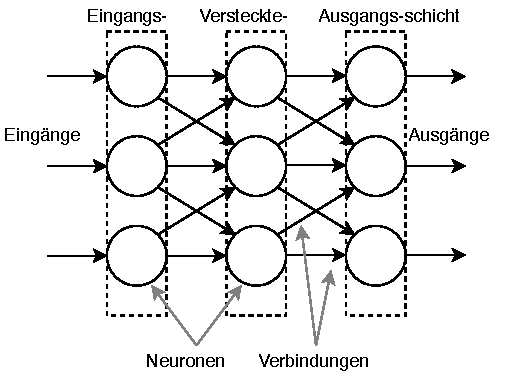
\includegraphics[scale=1.2]{img/mlp.pdf}
  \caption{Künstliches neuronales Netz mit drei Schichten je drei Neuronen}
  \label{fig:neural_network}
\end{figure}


\begin{itemize}
\item \textbf{Eingangsschicht} Die Neuronen der Eingangsschicht sind nicht wie die in \ref{Aufbau eines Neurons} beschriebenen Neuronen aufgebaut. Die einzige Aufgabe der Eingangsneuronen ist das Verteilen der Eingangsinformationen an die versteckte Schicht, weshalb es immer genau so viele Eingangsneuronen wie Eingangssignale geben muss.

\item \textbf{Versteckte Schicht}
Die versteckte Schicht (engl. hidden Layer) besteht aus den in \ref{Aufbau eines Neurons} erläuterten Neuronen. Sie kann aus einer beliebigen Anzahl von Neuronen aufgebaut sein. Es kann auch beliebig viele dieser Schichten geben. In der Literatur werden  neuronale Netze mit mehr als einer versteckten Schicht als Deep Neural Networks bezeichnet.

\item \textbf{Ausgangsschicht}
Die Ausgangsschicht beinhaltet genauso viele Neuronen wie Ausgangsgrößen gewünscht. Aus dieser können dann die Klassifizierungswerte entnommen werden.
\end{itemize}

\subsection{Verlustfunktion}
Die Verlustfunktion (engl. Lossfunction) stellt ein ausgesuchtes Maß der Diskrepanz zwischen den beobachteten und den vorhergesagten Daten dar. Sie bestimmt somit die Leistungsfähigkeit des künstlichen neuronalen Netzes während des Trainings. Beim Rückgabewert wird von dem Fehler (engl. loss) gesprochen.

\subsection{Fehlerrückführung}
Fehlerrückführung ist ein Optimierungsalgorithmus, welcher auf dem Gradientenabstieg basiert. Dies ist nur möglich, da ein KNN aus verketteten differenzierbaren Gewichten aufgebaut ist und somit die Kettenregel angewendet werden kann. Ziel ist es den Fehler der Verlustfunktion zu minimieren. Hierfür wird ein Muster am Eingang des Netzes angelegt. Der Ausgangswert wird mit dem Soll-Ergebnis verglichen. Der aufsummierte Fehler wird Schichtweise von der Ausgangsschicht zur Eingangsschicht zurück propagiert. Währenddessen werden die Gewichte so geändert, dass der Fehler minimiert wird. Es gibt verschiedene Ansätze der Fehlerrückführung, welche auch Optimierer genannt werden. Diese bestimmen die Regeln, wie die Verlustfunktion zur Aktualisierung der Parameter verwendet wird. \cite[p.~83]{Chollet2018}


\subsection{Hyperparameter} \label{sec:Grundlagen_Hyperparamete}
Als Hyperparameter werden in Bezug auf künstliche neuronale Netze meist die Anfangsparameter bezeichnet, welche zum Traininieren eines Netzes essenziell sind. Für diese gelten keine universellen Werte, sondern müssen je nach Daten und Modell speziell angepasst und verändert werden. Infolgedessen sind nur einige Regeln und grobe Abschätzungen bekannt, in welchen Grenzen sich die Hyperparameter befinden. Zu den Hyperparametern, welche in dieser Arbeit verwendet werden, gehören folgende:
\begin{itemize}
\item \textbf{Die Lernrate} ist das Maß für die Schrittgröße beim Gradientenabstieg. Eine zu kleine Lernrate kann zu einem sehr langsamen Training führen. Eine zu große Lernrate kann dazu führen, dass der Wert um ein Minimum oszilliert. Dies ist grafisch in Abbildung \ref{fig:learnrate} dargestellt. \cite[p.~49]{francois2017deep}
\begin{figure}[H]
  \centering  
  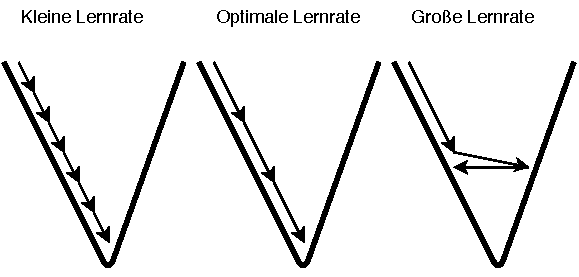
\includegraphics[scale=1]{img/learningrate.pdf}
  \caption{Links zu kleine Lernrate, mitte optimale Lernrate, rechts zu große Lernrate}
  \label{fig:learnrate}
\end{figure}

\item \textbf{Der Dropout} gibt an, wie viel Prozent einer Schicht während des Trainings deaktiviert werden. Deaktiviert bedeutet, diese werden ignoriert und für diese Iteration ausgesetzt. Symbolisch zu sehen in Abbildung \ref{fig:dropout}. Durch das deaktivieren werden zufällige Neuronen "`Null"' gesetzt, dadurch muss das Netz diese deaktivierten Neuronen durch andere Neuronen ersetzen, wodurch die Informationen, welche in den Neuronen gespeichert sind, besser verteilt werden. Dropout wird nur an den versteckten Schichten durchgeführt und kann zu einem verbesserten und robusteren Ergebnis führen\cite[p.~109]{francois2017deep}.

\begin{figure}[H]
  \centering  
  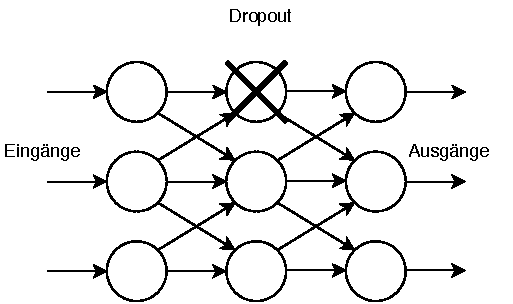
\includegraphics[scale=1]{img/dropout.pdf}
  \caption{Abdeckungsgrad entspricht einem Drittel}
  \label{fig:dropout}
\end{figure}

\item \textbf{Die Epochen} geben an, wie viele Iterationen aller Trainingsdaten durchgeführt werden sollen. Ein zu langes Training kann zu einem Auswendiglernen der Daten führen und dementsprechend wird nicht mehr richtig generalisiert. Bei einer zu geringen Epochen-Anzahl kann das Netz nicht genügend Informationen lernen, das Ergebnis ist dann entsprechend schlecht \cite[p.~109]{francois2017deep}.

\item \textbf{Die Batchsize} gibt an, in welchen Paketen die Daten dem künstlichen neuronalen Netz zugeführt werden. Künstliche neuronale Netze verarbeiten die Daten nicht auf einmal, sondern teilen sie in sogenannte Stapel ein\cite[p.~109]{francois2017deep}. 

\item \textbf{Der Optimierer} (engl. Optimizer) gibt vor, wie sich der Fehler auf die Aktualisierung der Parameter auswirkt. So gibt es beispielsweise einen stochastischer Gradientenabstieg mit Momentum Optimierer (engl. Stochastic Gradient Descent with momentum), der die Trägheit des Gradientenabstiegsverfahren berücksichtigt und damit besser lokale Minima über geht\cite[p.~109]{francois2017deep}. Die Erklärung aller Optimierer ist nicht Teil der Arbeit, es wird daher auf die Arbeit \cite{DBLP:journals/corr/Ruder16} verwiesen, in welcher die wichtigsten Optimierer ausführlich erklärt werden.

\item \textbf{Die Modell-Achitektur} definiert wie ein Netz aufgebaut ist. Hier werden die Anzahl der Schichten und Neuronen festgelegt. Ein zu kleines Netz kann nicht alle Informationen lernen, die in den Daten vorhanden sind. Dies zeigt sich schnell in schlechten Ergebnissen. Ein zu großes Netz mit zu vielen Schichten und Neuronen kann dazu führen, dass die Genauigkeit bei den Trainingsdaten steigt, was wiederum dazu führt, dass sich die Genauigkeit bei den Testdaten verschlechtert. Zudem ist die Dauer des Trainings wesentlich länger\cite[p.~70]{francois2017deep}. 
\end{itemize}


\section{Optimierung}
Als Optimierung wird im Allgemeinen die Maximierung oder Minimierung einer Zielfunktion bezeichnet, wobei eine oder mehrere Restriktionen eingehalten werden sollen. Hierbei existiert ein Lösungsraum, in dem sich sämtliche mögliche Lösungen befinden. Das Optimierungsverfahren soll den Lösungsraum definieren und diesen Lösungsraum nach der Lösung mit dem optimalen Zielfunktionswert absuchen \cite[p.~15]{Gerdts2011}. Bei der Hyperparameteroptimierung handelt es sich um ein Mehrzieloptimierungproblem, wodurch sich ein mehrdimensionaler Suchraum ergibt. Eine exakte Berechnung des Optimums ist, wegen des großen Suchraums, meist nicht möglich. Aus diesem Grund ist für diese Aufgabe nur eine heuristische Optimierung möglich. Bei heuristischen Verfahren wird der Lösungsraum nach einem festgelegten Muster durchsucht und bewertet. Die gefundenen Lösungen sind meist nicht die besten Lösungen, sind aber der Kompromiss aus vertretbarem Rechenaufwand und hinreichend gut eingeschätzter Lösung. Trotz allem kann nicht garantiert werden, dass es sich bei der gefunden Lösung um die optimale Lösung handelt\cite{beume2006mehrkriterielle}. Für diese heuristischen Verfahren zur Hyperparameter Optimierung werden in dieser Arbeit Zufallssuche und Genetischen Algortihmen gegenübergestellt und anhand ihrer Lösungen verglichen und bewertet.


\textbf{Vereinfachtes Beispiel für Mehrzieloptimerung}
Angenommen, es soll ein künstliches neuronales Netz mit k Schichten und j Neuronen zur Klassifizierung von einfachen handgeschriebenen Zahlen erstellt werden. Der Entwickler entscheidet sich für ein Netz mit 3 Schichten und jeweils 3 Neuronen. Nach dem Training hat das Netz eine Genauigkeit von 85 Prozent. Nun kann der Programmier/Entwickler nicht sicher sagen, ob für k = 3 und j = 3  die optimale Lösung gefunden wurde. Um dies beurteilen zu können, müssen viele Experimente durchgeführt werden. Die Frage dabei ist, wie die besten Werte für k und j zu finden sind, um die Klassifizierungsgenauigkeit maximieren zu können. Dieser Vorgang, speziell im Zusammenhang mit künstlichen neuronalen Netzen, wird als Hyperparameter-Optimierung bezeichnet. Bei der Optimierung wird mit einem Initialwert gestartet. Dieser ist in den seltensten Fällen die exakte Lösung und muss einige Male verändert werden, um auf ein Optimum zu gelangen. In dieser Arbeit ist dafür die Zufallssuche, bzw. der Genetische Algorithmus zuständig\cite[p.~130]{Gad2018}. 


\section{Rastersuche und Zufallssuche} \label{Zufalls_Suche}
Die Rastersuche(engl. Grid Search) ist einer der am weiterverbreiteten Optimierungsalgorithmen. Der Suchraum wird durch ein Raster aufgeteilt, je höher die Abtastrate desto feiner ist das Raster. Die Überschneidungen des Gitters sind im Endeffekt die einzelnen Punkte, welche getestet werden. Während des Suchvorgangs wird das Raster nicht verändert. Somit kann es passieren, dass die optimalsten Parameter nicht gefunden werden, zudem ist die Suche sehr langsam bzw. rechenaufwendig. Um eine schnellere Berechnung von Hyperparametern zu garantieren, wurde von James Bergtra und Yoshua Bengio die Zufallssuche untersucht. Sie konnten statistisch feststellen, dass die Zufallssuche schneller bessere Ergebnisse liefert. \cite{bergstra2012random} Wie in Abbildung \ref{fig:RandomSearch} zu sehen ist, ist die Abdeckung des Suchraums durch die Zufallssuche, auf der rechte Seite, wesentlich besser als die Rastersuche auf der linken Seite. Dies ist möglich, da die Zufallssuche zufällig innerhalb des Rasters sucht und nicht nur die Überschneidungen des vorgegebenen Rasters untersucht.

\noindent%
\begin{figure}
  \centering  
  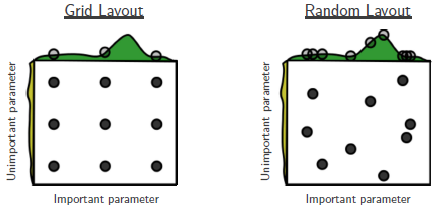
\includegraphics[scale=0.9]{img/gridsearch.png}
  \caption{Linke Seite: "Grid Search", Rechte Seite: "Random Search" \cite{bergstra2012random}}
  \label{fig:RandomSearch}
\end{figure}

\section{Genetische Algorithmen} \label{Genetische_Algorithmen}
Im folgenden Unterkapitel wird näher auf die 5 Schritte des Genetischen Algorithmus(GA) \ref{GA} eingegangen. Zuerst wird auf den Aufbau und die Initialisierung einer Population eingegangen. Anschließend folgt eine Zusammenfassung der Fitnessfunktion. Darauf folgend werden verschiedene Möglichkeiten für die Eltern Selektion dargelegt. Anschließend wird die Vermehrung durch Crossover und Mutation erklärt. Zum Schluss wird auf den Austausch der Populationen eingegangen. 

Genetische Algorithmen sind der Evolution von Darwin nachempfunden. Es geht hierbei um das ÜberlebeFon des Fittesten (engl. Survial of the Fittest) wobei es in dieser Arbeit nicht um das biologische Leben geht. Der Algorithmus ist der in der Natur vorkommenden Evolution ähnlich, weshalb auch viele Begriffe an die biologische Evolution angelehnt werden. Genetische Algorithmen sind heuristische Suchansätze. Im Wesentlichen zeichnet sie eine probabilistische Eltern Selektion als primären Suchoperator aus. Als weiterer Operator wird auf die Mutation zurückgegriffen. Dieser garantiert eine Erreichbarkeit aller Punkte im Suchraum und erhält die Grunddiversität in der Population. Es gibt zwei verschiedene Algorithmen, zum einen den Standard-GA, welcher nach einer Generation die komplette Elternpopulation durch die Kinderpopulation austauscht. Dieser besteht in der Regel immer aus den gleichen fünf Schritten: \\
Schritt 1, Initialisieren der Anfangspopulation. \\
Schritt 2, Fitness berechnen mit Hilfe der Fitnessfunktion. \\
Schritt 3, Selektieren der Eltern. \\
Schritt 4, Vermehren durch Crossover und Mutation. \\
Schritt 5, Austausch der Populationen. \\
Diese Schritte sind in Abbildung \ref{fig:Ablauf_kurz} noch einmal zum leichteren Verständnis als Flussdiagramm dargestellt.
Im Gegensatz dazu steht der Steady-State-GA, welcher sich durch eine überlappende Population auszeichnet. Pro Generation wird nur das schlechteste Individuum durch ein neues Individuum ausgetauscht. Der Steady-State-GA wird in der Arbeit nicht verwendet und wird deswegen nicht weiter erklärt, da er für die kleinen Suchräume geeignet ist. \cite[p.~128]{weicker2015evolutionare}  \cite[p.~11]{kramer2017genetic}. 

\noindent%
\begin{figure}[H]
  \centering  
  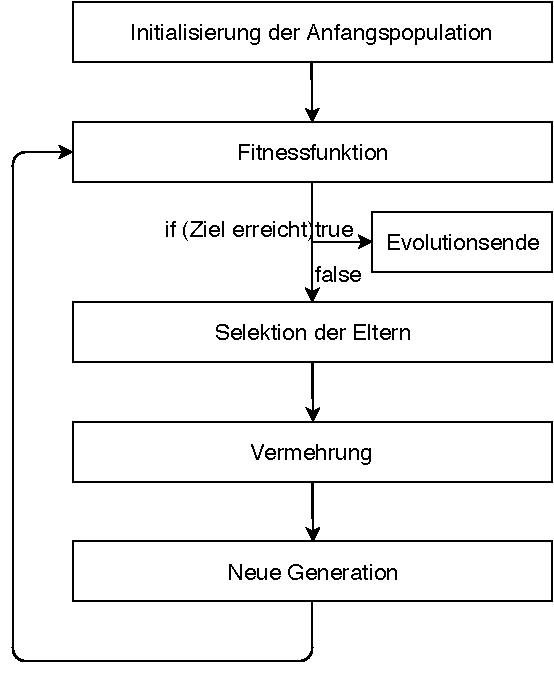
\includegraphics[scale=0.8]{img/Ablauf_kurz.pdf}
  \caption{Ablaufdiagramm eines genetischen Algorithmus mit 5 Schritten}
  \label{fig:Ablauf_kurz}
\end{figure}


\begin{algorithm}[h]
\SetAlgoLined
Initialisieren der Anfangspopulation\;
\While{$ Fitness \leq Abbruchbedingung$}{
 Fitness aller Individuen berechnen\;
 Selektieren der Eltern\;
 Vermehren durch Crossover und Mutation\;
 Austausch der Populationen\;
 }
\caption{Genetischer Algorithmus} \label{GA}
\end{algorithm}


\newpage
\subsection{Aufbau und Initialisierung  der Population}
Der klassische genetische Algorithmus basiert auf einer Reihe von Kandidatenlösungen. Die Größe der Population ist somit auch die Anzahl der Lösungen. Jede Lösung kann als einzelnes Individuum gesehen werden und wird durch einen Chromosomenstrang repräsentiert. Ein Chromosom besteht wiederum aus beliebig vielen Genen, wobei jedes Gen einen Parameter repräsentieren kann. Der Aufbau ist grafisch in Abbildung \ref{fig:population} dargestellt. Um die Grundlagen nahe, des später folgenden Konzepts zuhalten, wird der Ablauf per Dezimal-Genen erklärt\cite[p.~134]{Gad2018}. 


\noindent%
\begin{figure}[H]
  \centering  
  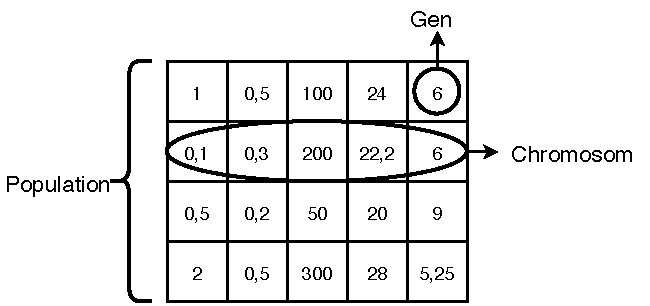
\includegraphics[scale=0.9]{img/population_ohne.pdf}
  \caption{Beispiel einer Population mit 4 Individuen (Chromosom) mit 5 dezimalen Genen}
  \label{fig:population}
\end{figure}

Diese Anfangspopulation (Generation 0) wird zufällig initialisiert, um die größtmögliche Abdeckung des Suchraums zu gewähren. Die erste Generation besitzt eine sehr geringe Fitness, welche sich im Verlauf des Trainings stetig steigert bis sie das Maximum erreicht.

\subsection{Fitnessfunktion}
Die Fitnessfunktion (engl. Fitnessfunction) bewertet das Individuum anhand seiner Funktionstauglichkeit, bezogen auf die vorhandene Aufgabe. Dabei wird das Chromosom (Individuum) als Ganzes bewertet, somit wird keine Aussage über einzelne Gene getroffen. Die Fitnessfunktion muss für jede Anwendung speziell geschrieben werden. Der Rückgabewert der Fitnessfunktion entspricht einer reellen Zahl. Ein höherer Fitnesswert steht immer für eine höhere Qualität des Individuums, bzw. eine bessere Lösung\cite[p.~135]{Gad2018}. 

\newpage

\subsection{Selektion der Eltern} \label{Grundlagen_eltern_selektion}
Bei dem Schritt Selektion der Eltern (engl. Select Parents) geht es, darum einen Elternpool zu generieren, aus welchem die neue Generation erstellt wird. Deshalb ist es wichtig, nur die qualitativ hochwertigsten Individuen auszuwählen. Es gibt verschiedene Ansätze bei der Selektion. Die elementar Wichtigsten werden im Folgenden genannt und erläutert. Informationen zu den Selektionsmethoden wurden aus den Arbeiten \cite{shukla15} \cite[p.~80]{eiben2003introduction} entnommen.

\begin{itemize}
\item \textbf{Auswahl proportional zur Fitness (engl. Fitness Proportionate Selection(FPS))} Die Eltern werden proportional nach ihrer Fitness ausgewählt und zum Elternpool hinzugefügt. $f(a_i)$ ist die Fitness des Individuums $a_i$ in der Population. $ps(a_i)$ ist die Wahrscheinlichkeit des Individuums, $a_i$ als Elternteil ausgewählt zu werden.
\begin{equation}
	ps(a_i) = \frac{f(a_i)}{\sum_{j=1}^n f(a_j)}; i\in{1,2,...,n} \label{eq:7}
\end{equation}
Wobei n die Anzahl der Individuen einer Population enstspricht.
Diese Wahrscheinlichkeit $ps$ wird als Anteil auf einem Rouletterad, wie Abblidung \ref{fig:roulette_wheel} zeigt, umgesetzt. Auf dem zufällig die Eltern aus den Individuen $a1,..,an$  "`ausgedreht"' werden. Dieser Ansatz hat leider das Problem, dass Individuen, welche sich am Anfang als gut beweisen, schnell die ganze Population übernehmen. Dies kann dazu führen, dass eine mögliche bessere Lösung durch den Algorithmus im Suchraum nicht gefunden wird.

\begin{figure}[htb]
  \centering  
  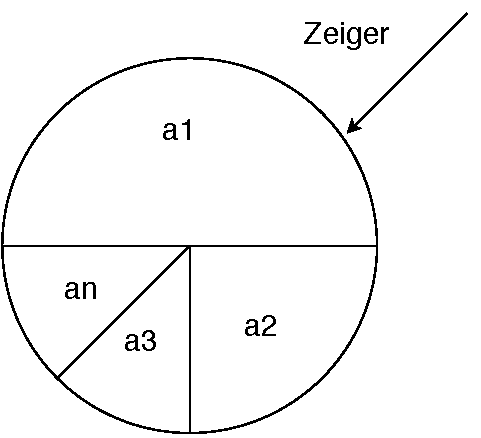
\includegraphics[scale=0.7]{img/roulette_wheel.pdf}
  \caption{Rouletterad mit proportionalem Anteil der Individuen anhand ihrere Fitness}
  \label{fig:roulette_wheel}
\end{figure}


\item \textbf{Ranking Selektion} Diese Selektion wurde von Backer als Verbesserung der Fitness proportional Selection entwickelt \cite{baker1985adaptive}. Dabei werden die Eltern nicht direkt nach ihrer Fitness ausgewählt. Die Fitness dient nur zum Einteilen in eine Rangliste. Anhand dieser Rangliste wird nun die Verteilung auf dem q berechnet. Dazu gibt es zwei Ansätze:

Das lineare Ranking:
\begin{equation}	
	p_i = \frac{1}{N}(n^- + (n^+ - n^- ) \frac{i-1}{N-1}; i\in{1,...,N} \label{eq:8}
\end{equation}
Wobei $p_i$ die Wahrscheinlichkeit des Individuums ist, selektiert zu werden. $\frac{n^-}{N}$ ist die Wahrscheinlichkeit, des schlechtesten Individuums selektiert zu werden und  $\frac{n^+}{N}$ ist die Wahrscheinlichkeit, des besten Individuums selektiert zu werden.

Das exponentielle Ranking:
\begin{equation}
	p_i = \frac{c^{N-i}}{\sum_{j=1}^N c^{N-j}}; i\in{1,...,N} \label{eq:9}
\end{equation}
die Summe $\sum_{j=1}^N c^{N-j}$ normalisiert die Wahrscheilichkeit um Sicherzustellen, dass $\sum_{i=1}^N p_i = 1$.
Wobei die Berechnungen \ref{eq:8} und \ref{eq:9} nur den Anteil eines Individuums auf dem Rouletterad verändern.

\item \textbf{Turnier Selektion} In diesem Verfahren, welches in Abbildung \ref{fig:tunier} zusehen ist, werden zufällig k Individuen der Population ausgewählt. Diese k Individuen treten wie in einem Turnier gegeneinander an. Der Gewinner ist das Individuum mit dem besten Fitnesswert, dieser wird dann auch als Elternteil ausgewählt. Hierbei wird auf den Elternpool verzichtet und direkt ein Kind aus zwei Gewinnern erstellt. Eingesetzt wird dies bei kleineren Populationen mit weniger als 20 Individuen.

\begin{figure}[htb]
  \centering  
  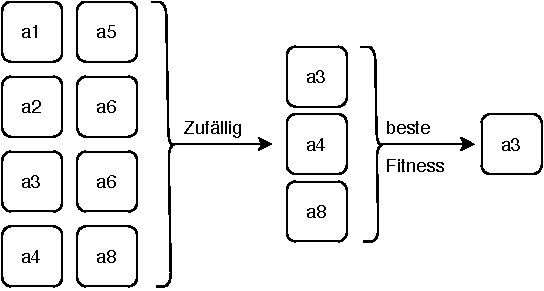
\includegraphics[scale=0.8]{img/tunier.pdf}
  \caption{Turnier Selektion mit k = 3 Individuen und dem Gewinner Individuum 3}
  \label{fig:tunier}
\end{figure}


\end{itemize}


\subsection{Vermehrung} \label{Grundlagen_vermehrung}
Aus dem Elternpool werden nun Nachkommen (neue Individuen) geschaffen. Alleine durch die Paarung(engl. Crossover) von qualitativ hochwertigen Individuen wird erwartet, dass die Nachkommen eine bessere Qualität besitzen als die ihrer Eltern. Als zweite Verbesserung wird noch die Mutation einzelner Gene angewendet. In diesem Abschnitt werden die verschiedenen Ansätze für Crossover und Mutation näher erklärt.

\paragraph{Crossover} Hierbei werden aus zwei Eltern Chromosomen, die Chromosomen der Kinder zusammengesetzt. Informationen zu Crossover wurden aus der Arbeit \cite{Umbarkar2015} entnommen. Die bedeutendsten Cossover-Varianten sind:

\begin{itemize}
\item \textbf{One-Point-Crossover}
Bei Ein-Punkt-Crossover wird zufällig ein Punkt im Chromsomenstrang festgelegt. Ab diesem Punkt wird der Chromosomenstrang dann aufgeteilt und anschließend mit dem Crossover des anderen Elternteils zusammengesetzt. Ein einfaches Beispiel ist im oberen Teil der Abbildung \ref{fig:chromoson_crossover} zu sehen.

\item \textbf{k-Point-Crossover}
Eine Abwandlung des Ein-Punkt-Crossover ist das Zwei-Punkt-Crossover oder k-Punkt-Crossover. Hier wird der Chromsomenstrang an k Punkten aufgeteilt und anschließend mit dem Anteil des zweiten Elternteil wieder zusammengesetzt. Im mittleren Teil der Abbildung \ref{fig:chromoson_crossover} ist ein k = 2 Crossover oder auch zwei-punkt-crossover (engl. two-point-crossover) zu sehen.

\item \textbf{Uniform-Crossover}
Eine weitere grundlegende Operation beim Crossover ist die Uniform-Crossover \cite{Syswerda1989}. Hier wird für jedes Gen zufällig entschieden aus welchem Elternteil das Gen entnommen wird. Dies ist im unteren Teil der Abbildung \ref{fig:chromoson_crossover} veranschaulicht.
\end{itemize}

\begin{figure}[H]
  \centering  
  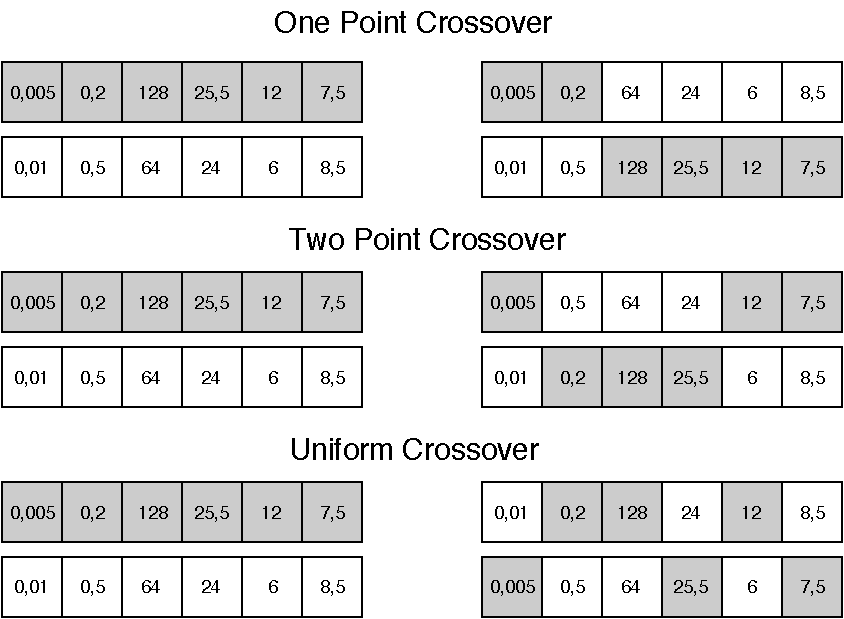
\includegraphics[scale=0.8]{img/crossover_gene.pdf}
  \caption[Crossover Varianten]{Die wichtigsten drei Crossover Operationen: oben one-point Crossover, mitte two-point Crossover, unten Uniform Crossover. Auf der linken Seite sind die Eltern abgebildet und auf der rechten Seite die neu erzeugten Kinder}
  \label{fig:chromoson_crossover}
\end{figure}


\paragraph{Mutation} Hierbei wird jedes Gen des Individuums zufällig mit einer zufälligen Mutation versehen. Zum einen gibt es eine einstellbare Wahrscheinlichkeit, ob ein Gen verändert werden soll und zum anderen wie groß die Mutation sein soll. Durch diese Mutation wird eine höhere Diversität in die nachfolgende Generation übergeben. Diese Mutation macht es möglich, einen größeren Suchraum abzudecken und somit die Werte genauer anzupassen, um so auf die optimale Lösung zu kommen. Es wird ein Zufallswert aus der Normal- oder Gauß-Verteilung zum Gen hinzuaddiert. Durch diese Wahrscheinlichkeitsverteilung erhalten viele Gene nur kleine Veränderungen, aber auch größere Mutationen sind möglich. Um die vorher mit Crossover neu bestimmten Individuen, welche schon eine hohe Grundfitness besitzen, nicht zu stark zu verändern, wird ein Gen nur um wenige Prozent verändert. Dies ist in Abbildung \ref{fig:chromoson_mutation} zu sehen\cite[p.~60]{weicker2015evolutionare} \cite[p.~140]{Gerdts2011}. 

\begin{figure}[H]
  \centering  
  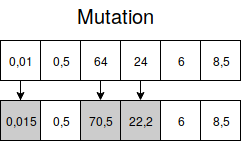
\includegraphics[scale=0.9]{img/mutation.png}
  \caption{Beispielhafte, zufällige Mutation}
  \label{fig:chromoson_mutation}
\end{figure}

 
\subsection{Neue Generation}
Der letzte Schritt des Genetischen Algorithmus besteht aus dem Austausch der Generationen. Die neue Kind-Generation tauscht nun die alte Eltern-Generation aus. Anschließend folgen die gleichen 4 Schritte so lange, bis der gewünschte Fitnesswert erreicht ist. Nach dem Erreichen der Abbruchbedingung, kann aus der letzten Generation das qualitativ hochwertigste Individuum ausgesucht und als Lösung verwendet werden.


\section{Zusammenfassung}
In diesem Kapitel wurden die Grundlagen erklärt, welche zum Verständnis dieser Arbeit notwendig sind. Zuerst wurden die künstlichen neuronalen Netze erklärt, welche dem Aufbau des menschlichen Gehirns gleichen. Das KNN kann aus den Daten so lineare, als auch nicht lineare zusammenhänge erlernen. Des Weiteren wurde der Genetische Algorithmus und die Zufallssuche erklärt. Bei beiden handelt es sich um Optimierungsalgorithmen für eine Mehrzieloptimierung. Die Zufallssuche ist ein zufälliges abtasten innerhalb eines Suchraums. Der Genetische Algorithmus ist der Evolution von Charles Darwin nachempfunden. Er basiert auf dem Prinzip des "`Survival of the Fittest"', dies bedeutet, dass die besten Individuen sich durchsetzen und aus diesen mit Crossover und Mutation eine neue Generation erstellt wird.